\documentclass[12pt,a4paper,titlepage]{article}

\usepackage[utf8x]{inputenc}
\usepackage{ucs}
\usepackage[portuguese]{babel}
\usepackage[T1]{fontenc}
\usepackage{amsmath}
\usepackage{amsfonts}
\usepackage{amssymb}
\usepackage{graphicx}
\usepackage{fancyhdr}
\usepackage{lastpage}
\usepackage{geometry}
\usepackage{float}
\usepackage{makecell}
\usepackage{multirow}
%\usepackage{hyperref}
\usepackage[table,xcdraw]{xcolor}
%\usepackage{caption}
%\usepackage{subcaption}
%\usepackege[nogin]{sweave}



\usepackage{Sweave}
\begin{document}
\Sconcordance{concordance:exercicio5.tex:exercicio5.Rnw:%
1 24 1 1 0 16 1 1 15 1 37 39 0 1 2 4 1 1 51 80 0 1 2 38 1}


\begin{center}
{\huge KMeans}

{\large Victor Marcius Magalhães Pinto}
\end{center}

\section{Descrição da Tarefa}

O exercício consiste em aplicar o algoritmo \textit{k-Means} para realizar a obtenção de um agrupamento de clusters de features, através da concatenação de gaussianas no espaço. Para tanto, foram criados quatro agrupamentos de clusters, que consistem em distribuições gaussianas bidimensionais.

\section{Execução do Código}

A função k-Means implementada consistem em.


\begin{Schunk}
\begin{Sinput}
> kMeans <- function (X, k, maxit) {
+   N <- dim(X)[1]
+   n <- dim(X)[2]
+   
+   seqN <- seq(1,N,1)
+   seqk <- seq(1,k,1)
+   
+   Mc <- matrix(nrow=k, ncol=n)
+   Clustx <-matrix(nrow=N, ncol=1)
+   
+   seqx <- sample(N,k)
+   
+   Mc <- X[seqx,]
+   
+   it <- 1
+   
+   while(it <= maxit){
+     for (i in seqN) {
+       xrep <- matrix(X[i,], nrow=k, ncol=n, byrow=T)
+       vecdist <- rowSums((Mc-xrep)^2)
+       Clustx[i] <- which.min(vecdist)
+     }
+     
+     for (j in seqk) {
+       xj <- which(Clustx==j)
+       Mc[j,] <- colMeans(X[xj,])
+     }
+     it <- it+1
+   }
+   
+   nam <- c("Mc","Clustx")
+   retlist <- list(Mc,Clustx)
+   names(retlist) <- nam
+   
+   return(retlist)
+ }
\end{Sinput}
\end{Schunk}

A função é responsável por calcular os centros dos clusters, e de devolver o cluster correspondente de cada uma das amostras, segundo a distribuição de probabilidade correspondente.

Para testarmos o código, realizamos a execução do mesmo para os 4 grupamentos de clusters, variando o desvio padrão de cada um deles, entre 0.3, 0.5 e 0.7, além de variar a quantidade de centros considerados, entre 2, 4 e 8, ou seja, com menos clusters que o considerado, com o número de clusters criados, e com mais clusters do que existentes. A execução foi realizada em loops, e o resultado pode ser visto abaixo.

\begin{Schunk}
\begin{Soutput}
>> Centros para k =  2 e desvio padrão de  0.3 .

                   x1         x2
centro  1 :  2.984316  3.0242786
centro  2 : -1.011185 -0.9685763

>> Centros para k =  4 e desvio padrão de  0.3 .

                     x1           x2
centro  1 :  0.01171457  0.006367283
centro  2 :  1.96363308  1.999802260
centro  3 : -2.00846950 -2.005238772
centro  4 :  4.02018294  3.942545103

>> Centros para k =  8 e desvio padrão de  0.3 .

                    x1          x2
centro  1 :  2.0068580  1.73977881
centro  2 :  0.3334253 -0.16949846
centro  3 : -1.9183701 -1.99931337
centro  4 :  1.7305075  2.19753648
centro  5 :  3.9889649  3.97828588
centro  6 :  2.2936616  2.12561482
centro  7 : -0.3454421 -0.02149794
centro  8 :  0.1133806  0.21805037

>> Centros para k =  2 e desvio padrão de  0.5 .

                   x1        x2
centro  1 :  3.027628  2.935133
centro  2 : -1.047699 -1.019231

>> Centros para k =  4 e desvio padrão de  0.5 .

                    x1          x2
centro  1 :  0.1823524 -0.03035959
centro  2 :  4.0529942  4.10425252
centro  3 :  1.9566624  1.87139609
centro  4 : -1.9980825 -2.04126819

>> Centros para k =  8 e desvio padrão de  0.5 .

                    x1          x2
centro  1 :  3.2799540  3.61632653
centro  2 : -2.0503809 -2.20762573
centro  3 :  3.7101634  4.31067716
centro  4 :  4.3162104  3.56514781
centro  5 :  4.5181393  4.36708981
centro  6 : -0.0263776 -0.02697853
centro  7 : -1.8967553 -1.42292629
centro  8 :  1.9053243  2.07457332

>> Centros para k =  2 e desvio padrão de  0.7 .

                   x1        x2
centro  1 :  2.986613  3.010484
centro  2 : -1.105804 -1.160586

>> Centros para k =  4 e desvio padrão de  0.7 .

                    x1         x2
centro  1 :  0.3204529  0.1766506
centro  2 : -1.5440370 -2.3990022
centro  3 : -2.1712127 -1.3943933
centro  4 :  3.3383185  3.1701635

>> Centros para k =  8 e desvio padrão de  0.7 .

                    x1         x2
centro  1 :  1.7860927  2.2454379
centro  2 :  2.6295388  1.3713683
centro  3 :  0.4559780 -0.2988788
centro  4 :  4.0550168  4.5853445
centro  5 :  4.4265495  3.3894731
centro  6 : -2.0655447 -1.9396234
centro  7 : -0.5404434  0.3645965
centro  8 :  3.1335875  3.5306931
\end{Soutput}
\end{Schunk}

Os gráficos dos clusters correspondentes podem ser vistos a seguir.

\begin{figure}[H]
\centering
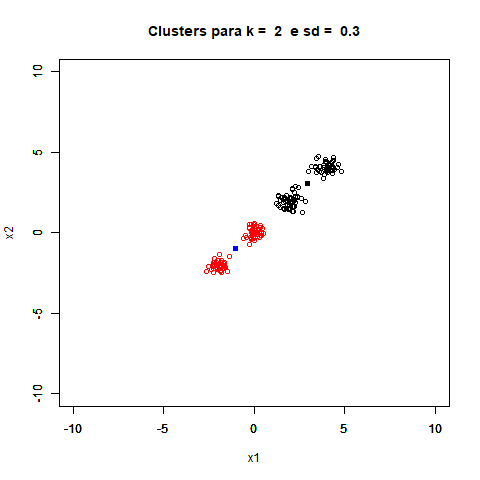
\includegraphics[width=0.3\linewidth]{k2sd03.png}
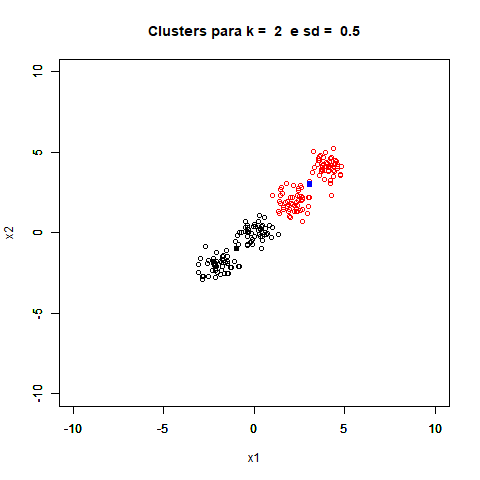
\includegraphics[width=0.3\linewidth]{k2sd05.png}
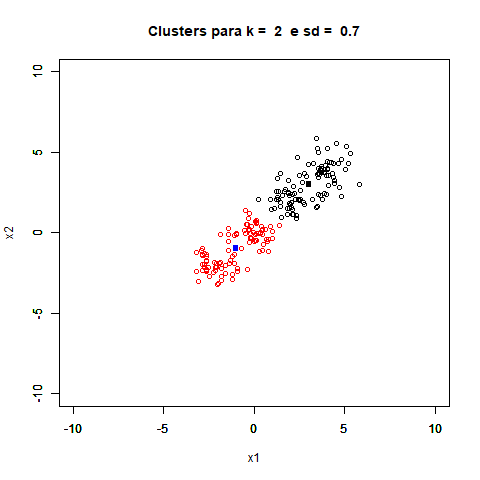
\includegraphics[width=0.3\linewidth]{k2sd07.png}

\caption{Distribuição dos clusters, e os centros correspondentes para k=2.}
\end{figure}

\begin{figure}[H]
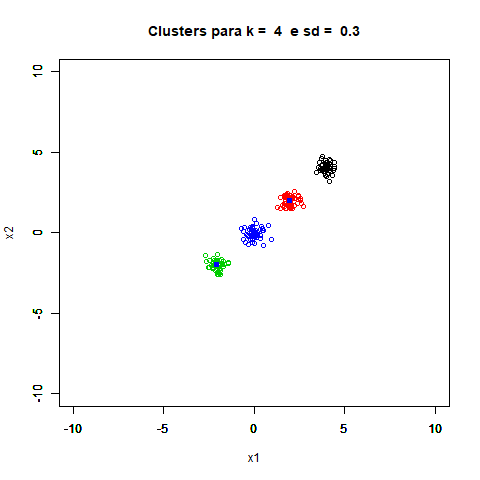
\includegraphics[width=0.3\linewidth]{k4sd03.png}
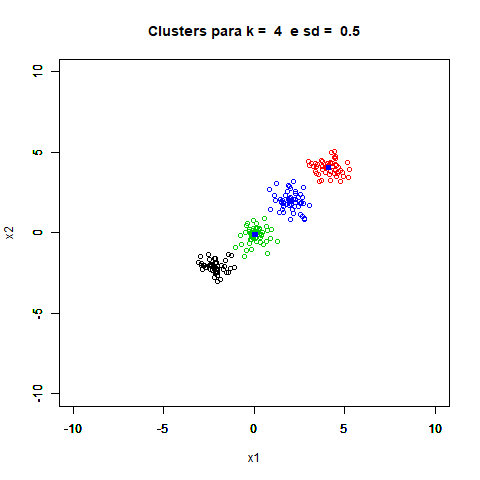
\includegraphics[width=0.3\linewidth]{k4sd05.png}
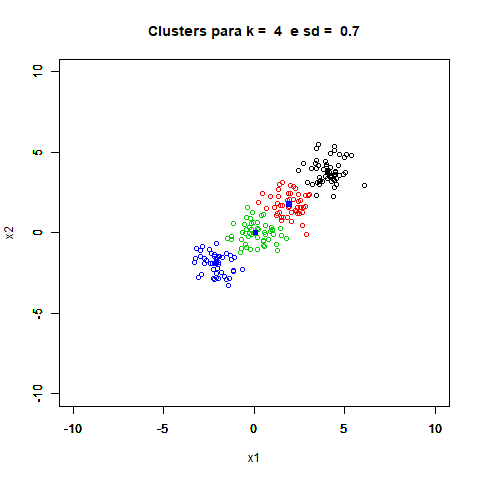
\includegraphics[width=0.3\linewidth]{k4sd07.png}
\caption{Distribuição dos clusters, e os centros correspondentes para k=4.}
\end{figure}

\begin{figure}[H]
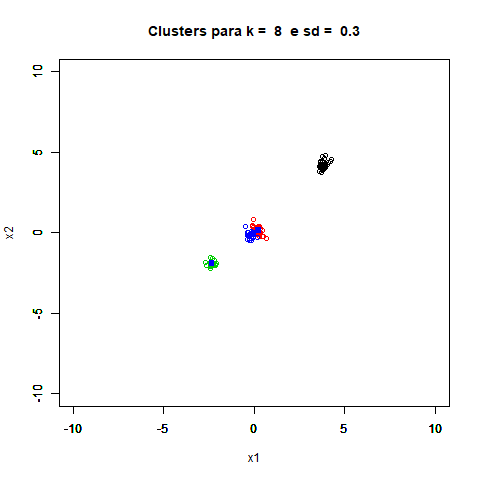
\includegraphics[width=0.3\linewidth]{k8sd03.png}
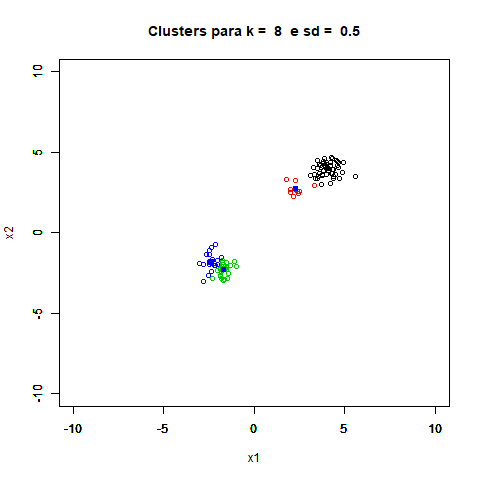
\includegraphics[width=0.3\linewidth]{k8sd05.png}
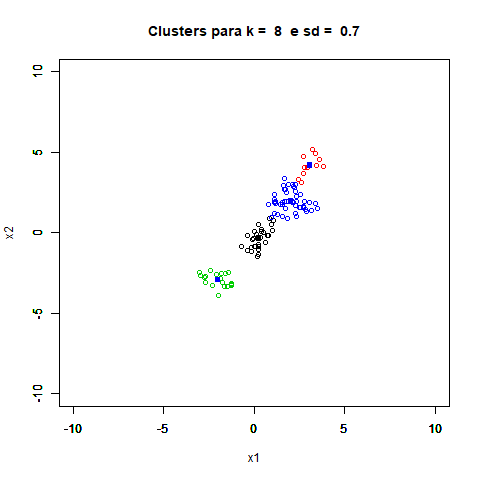
\includegraphics[width=0.3\linewidth]{k8sd07.png}
\caption{Distribuição dos clusters, e os centros correspondentes para k=8.}
\end{figure}

\section{Análise dos Resultados}

Como é possível ver para os gráficos, para o caso onde passamos para a função um k menor do que a quantidade de clusters exixtentes, o algoritmo reconhece como centros os pontos entre os clusters, ou seja, ele agrupa de dois em dois, e reconhece pontos intermediários como sendo os centros de cada um dos clusters.

Para o caso de k=4, ou seja, quando passamos corretamente para o algoritmo a quantidade de centros existentes, considerando a quantidade de clusters, temos que o algoritmo consegue identificar corretamente os centros dos agrupamentos.

No caso onde passamos mais centros do que os agrupamentos existentes, temos centros sendo estabelecidos em pontos próximos, e uma indentificação errônea das amostras, conforme poder ser visto nos plots correspondentes.

Não foi possível identificar nenhuma anomalia de funcionamento do algoritmo caso variemos o desvio padrão das amostras. Ele consegue identificar corretamente os centros para os clusters.

Portanto, podemos concluir que o algoritmo cumpre bem seu propósito de identificar os centros de cada agrupamento de amostras, contanto que não passemos para o mesmo uma quantiadade de centros que devem ser estabelecidos maior do que a separação dos clusters. Para estes casos, os centros extras são calculados próximos aos centros já existentes, sendo, portanto, redundantes.

\end{document}
